%!TEX root = ../../main.tex

\section{Reactive Synthesis}
\label{sec:reactive-synthesis}

Finally, we have reached the main topic of my thesis: Reactive Synthesis.

Reactive synthesis is the problem of translating a logical specification into a reactive system that is guaranteed to satisfy the specification for all possible behaviors of its environment. 
It differs from LTL Model Checking by the fact that we are not interested in figure out whether a given property $\phi$ holds in a model $\model$, but we want to generate a model $\model'$ automatically such that $\model' \models \phi$ by construction. 
In this case we say that the synthesized model $\model'$ is correct by construction.
Such model is a reactive system because its output is determined by reacting to the input values and formulated as either a Mealy Machine or a Moore Machine. 
The problem was introduced by Alonzo Church more than $60$ years ago \cite{C64}. 
Recent years have brought advances both in reasoning methods that can be used as tools in the synthesis process and in the synthesis approaches themselves.
As a result, the complexity of the synthesized systems has risen steadily. 
However, the logical and algorithmic foundations of the synthesis problem are still far from complete.

All algorithms to solve the Reactive Synthesis problem are based on game theory, in particular we can look at such problem like a two-players infinite games on finite graphs (\cite{R68}, \cite{W95}, \cite{BL90}). 
The main player is called Controller, or $P_0$, while the other player is called Environment, or $P_1$. 
Each player has a set of variables that can control and, since the game is seen from the perspective of $P_0$, the variables controlled by $P_0$ are called controllable and the ones controlled by $P_1$ are called uncontrollable.
In this type of games, it is chosen a-priori who performs the first move. 
It could be that $P_0$ moves first, it could be that $P_1$ moves first, or it could be that $P_0$ and $P_1$ move simultaneously. 
Along all the thesis we assume that $P_1$, the Environment, moves first and that every synthesized model is a Mealy Machine.

Let us start defining the Reactive Synthesis problem formally. 
In the following definition there are a lot of terms that could be unknown at first glace, but no worries because they are explained in the next sub-sections.

\begin{definition}[\cite{jacobs2015} Reactive Synthesis problem]
Let $\phi$ be a temporal formula over the alphabet $\Sigma = \C \cup \U$. We say that $\phi$ is realizable if and only if there exists a strategy $g \colon (2^\U)^+ \to 2^\C$ such that $U = \tuple{U_0,U_1,\dots} \in (2^\U)^\omega$, it holds that $g(U) \models \phi$. 
The synthesis problem is the decision problem to say whether $\phi$ is realizable or not. If $\phi$ is realizable, the corresponding strategy $g$ is computed.
\end{definition}

\subsection{Infinite game on graphs}
As we have already said previously, the reactive synthesis problem is reduced to infinite games on graphs.
There are some basic concepts which must be fixed before moving forward, in particular: the concept of an arena, what a strategy is, the concept of game and what we mean with winning region.

An \textit{arena} is the battlefield where two players clash. It is a finite graph, therefore it has some vertices and edges, and each player controls a subset of vertices. Controlling a vertex means to be able to select the edge and so the next vertex.   
Note that there are no vertices controlled by both players at the same time.
Whenever the two players play, they define the so called \textit{play} of the arena, which consists in the sequence of vertices crossed during the game. 
During the game both players do not act with out any logic, but they follow a \textit{strategy}. Such strategy is basically a function reading the play made so far, i.e. the sequence of vertices crossed so far, and select the next vertex to go. 
A strategy is called \textit{positional}, or memoryless, if the next vertex is chosen according to the current vertex and no the previous ones. 

\begin{definition}[\cite{infinite-games} Arena]
An arena $\arena = (V, V_0, V_1, E)$ consists of:
\begin{itemize}
    \item a finite set $V$ of vertices;
    \item disjoint subsets $V_0,V_1 \subseteq V = V_0 \cup V_1$ denoting the vertices of Player 0 and Player 1 respectively, and
    \item a set $E \subseteq V \times V$ of directed edges such that every vertex has at least one outgoing edge, i.e. $\set{v' \; | \; (v,v') \in E}$ is non-empty for every $v \in V$.
\end{itemize}
\end{definition}

\begin{definition}[\cite{infinite-games} Play]
A play in an arena $\arena = \tuple{V, V_0, V_1, E}$ is an infinite sequence $\rho=\rho_0\rho_1\rho_2\dots \in V^\omega$ such that $(\rho_n,\rho_{n+1}) \in E$ holds for every $n \in \Nat$. 
The set of plays in $\arena$ is denoted by $Plays(\arena)$, the set of all plays starting in $v$ by $Plays(A,v)$, and we define $Plays(A,V')=\bigcup_{v\in V'} Plays(\arena,v), \; \forall V' \subseteq V$.
\end{definition}

\begin{definition}[\cite{infinite-games} Strategy]
A strategy for Player $i \in \{0,1\}$ in an arena $\arena = \tuple{V,V_0,V_1,E}$ is a function $\sigma \colon V^*V_i \to V$ such that $\sigma(wv)=v' \implies (v,v') \in E,\; \forall w \in V^*,\; \forall v \in V$. 
\end{definition}

\begin{definition}[\cite{infinite-games} Consistent Play]
A play $\rho = \rho_0\rho_1\rho_2\dots$ in an arena $\arena=\tuple{V,V_0,V_1,E}$ is consistent with a strategy $\sigma$ for Player $i$ in $\arena$ if, $\rho_{n+1} = \sigma(\rho_0\dots\rho_n)$ for every $n \in \Nat$ with $\rho_n \in V_i$. 
Given a vertex $v$, we denote the set of plays that are consistent with $\sigma$ and start in $v$ with $Plays(\arena, v, \sigma)$. 
Finally, we define $Plays(\arena, V', \sigma)$ for $V'\subseteq V$ by $Plays(\arena, V', \sigma) = \bigcup_{v \in V'} Plays(\arena, v, \sigma)$.
\end{definition}

\begin{definition}[\cite{infinite-games} Positional (Memoryless) Strategy]
A strategy $\sigma$ for Player $i$ in an arena $\arena=(V,V_0,V_1,E)$ is positional (or memoryless) if $\sigma(wv)=\sigma(v)$ for all $w \in V^*$ and $v \in V$. 
Equivalently, a positional strategy can be seen as a function $\sigma \colon V_i \to V$.
\end{definition}

Only the arena is not enough to play a \textit{game}, but we need a winning condition.
When we set the winning condition, we call \textit{winning strategies} all those strategies which allow to win. 
The concept of winning strategies is connected to the one of \textit{winning region}, that is the set of all vertices starting from which a player has a winning strategy.
Therefore, we can reduce the reactive synthesis problem to find such winning region and, if it exists, then extract a strategy from it.

\begin{definition}[\cite{infinite-games} Game]
A game $\game=\tuple{\arena,Win}$ consists of an arena $\arena$ with vertex set $V$ and a set of winning sequences $Win \subseteq V^\omega$. 
We call a sequence $\rho$ winning for Player $0$ if and only if $\rho \in Win$ and winning for Player $1$ otherwise.
\end{definition}

\begin{definition}[\cite{infinite-games} Winning strategy]
Let $\game=(\arena,Win)$ be a game. A strategy $\sigma$ for Player $i$ in $\arena$ is a winning strategy from a vertex $v \in V$ if every play that is consistent with $\sigma$ and starts in $v$ is winning for Player $i$, i.e. if $Plays(\arena, v, \sigma) \subseteq Win$ for $i=0$ and $Plays(\arena, v, \sigma) \subseteq V^\omega \setminus Win$ for $i=1$. 
\end{definition}

\begin{definition}[\cite{infinite-games} Winning region]
The winning region $W_i(\game)$ of Player $i$ in a game $\game$ is the set of vertices from which Player $i$ has a winning strategy.
\end{definition}

\begin{definition}[\cite{infinite-games} Determinancy and Positional Determinancy]
Let $\game$ be a game with vertex set $V$. We say that $\game$ is determined if $W_0(\game)\cup W_1(\game) = V$. Furthermore, we say that $\game$ is positionally determined if, from every vertex $v \in V$ one of the players has a positional winning strategy.
\end{definition}

\begin{definition}[\cite{infinite-games} Uniform Positional Winning Strategy]
Let the game $\game=(\arena, Win)$. A strategy $\sigma$ for Player $i$ is a uniform positional winning strategy if it's positional and winning from every vertex in $W_i(G)$.
\end{definition}

\begin{figure}
    \centering
    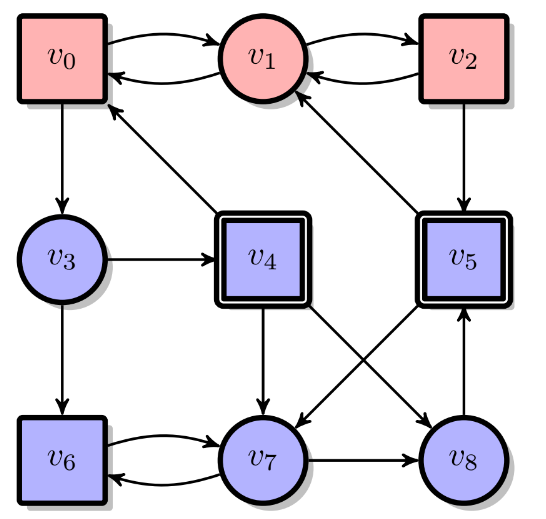
\includegraphics[width=0.4\linewidth]{figures/arena-example.png}
    \caption{\cite{infinite-games} Example of arena. The winning condition of player $0$ is to reach doubly-lined framed vertices (reachability game). Circular vertices are controlled by $P_0$, while rectangular ones are controlled by $P_1$. Blue and red vertices are $P_0$ and $P_1$ winning regions, respectively}
    \label{fig:enter-label}
\end{figure}

% \begin{lemma}
% For any game $\game$, it holds that $W_0(\game) \cap W_1(\game) = \emptyset$. In other words, the winning region of a player $i$ is the complement of the winning region for the player $1-i$, i.e. $W_i(\game) = V \setminus W_{1-i}(\game)$.
% \end{lemma}


\subsection{Safety and Reachability games}
The easiest games to solve, but at the same time enough interesting to analyze, are safety and reachability games.
Safety games consists in a game on an arena where we want to stay forever in a subset of vertices of the arena. In this case $P_0$ tries to stay forever in such subset, while $P_1$ tries to reach an outer vertex.
Reachability games consists in a game on an arena where we want to reach a subset of vertices of the arena. In this case $P_0$ tries to reach such subset, while $P_1$ tries to prevent $P_0$ to reach it by staying forever in the complement subset of vertices.

As maybe you could notice, safety and reachability games are dual: when $P_0$ is playing a safety game, $P_1$ is playing a reachability game, while when $P_0$ is playing a reachability game, $P_1$ is playing a safety game.

\begin{definition}[\cite{infinite-games} Occurrence set]
Given a play $\rho$, we denote as $Occ(\rho)$ the set of vertices occurring in $\rho$.
\end{definition}

\begin{definition}[\cite{infinite-games} Reachability game]
Let $\arena=\tuple{V, V_0, V_1, E}$ be an arena and let $R \subseteq V$ be a subset of $\arena$'s vertices. Then, the reachability condition $Reach(R)$ is defined as
\begin{flalign*}
    Reach(R) = \set{\rho \in V^\omega \; |\; Occ(\rho) \cap R \neq \emptyset}
\end{flalign*}
We call a game $\game = (\arena, Reach(R))$ a reachability game with reachability set $R$.
\end{definition}

\begin{definition}[\cite{infinite-games} Safety game]
Let $\arena = \tuple{V, V_0, V_1, E}$ be an arena and let $S \subseteq V$ be a subset of $\arena$'s vertices. Then, the safety condition $Safety(S)$ is defined as 
\begin{flalign*}
    Safety(S) = \set{\rho \in V^\omega \; | \; Occ(\rho) \subseteq S}
\end{flalign*}
We call a game $\game = (\arena, Safety(S))$ a safety game with safety set $S$.
\end{definition}

\begin{definition}[\cite{infinite-games} Dual Arena]
Let $\arena = \tuple{V,V_0,V_1,E}$ be an arena. The dual arena $\bar{\arena}$ of $\arena$ is defined as $\bar{\arena} = \tuple{V,V_1,V_0,E}$. 
\end{definition}

\begin{theorem}[\cite{infinite-games} Duality between safety and reachability games]
Let $\arena = \tuple{V,V_0,V_1,E}$ be an arena, let $\game = \tuple{A, SAFETY(S)}$ be a safety game with $S \subseteq V$ and define the reachability game $\game' = \tuple{\bar{\arena}, REACH(V \setminus S)}$. Then $W_i(\game) = W_{1-i}(\game')$ for each $i \in \set{0,1}$.
\end{theorem}

Let us now speak about algorithms to solve safety and reachability games. 
First of all, permit us to introduce some basic algorithms for solving such games on an explicit representation of the arena.
Afterwards, we will see that such algorithms can be empowered by BDD solving the games expressing the arena symbolically,

The fundamental algorithm to solve reachability is an algorithm based on fix-point computation of the 0-attractor. 
Basically, fixed a subset $R \subseteq V$ that we want to reach, we start computing the set of vertices from which the player $P_0$ can force to visit $R$ and $P_1$ can not avoid to visit $R$. Given such set of vertices we union with $R$ and do the same computation but now instead of reaching just $R$, we want to reach the new set resulting from the previous union. Going on like that we reach a point where the new computed set is not increasing anymore. 
That is the so-called fixed-point. 
We are sure to reach it because the set of vertices is finite.

\begin{definition}[\cite{infinite-games} i-Attractor]
Let $\game = (\arena, Reach(R))$ be a reachability game, where $\arena = \tuple{V, V_0, V_1, E}$ and $R \subseteq V$, and let $i \in \set{0,1}$ determine a player.
The controlled predecessor $CPre_i(R)$ of $R$ is defined as
\begin{flalign*}
CPre_i(R) = & \set{v \in V_i \; | \; \text{$v' \in R$ for some successor $v'$ of $v$}}\;\cup \\
            & \set{v \in V_{1-i} \; | \; \text{$v' \in R$ for all successors $v'$ of $v$}}
\end{flalign*}
The i-Attractor $Attr_i(R)$ in $\arena$ is defined by inductively applying the controlled predecessor via
\begin{flalign*}
& Attr_i^0(R) = R \\
& Attr_i^{n+1}(R) = Attr_i^n(R) \cup CPre_i(Attr_i^n(R)) \\
& Attr_i(R) = \bigcup_{n \in \Nat} Attr_i^n(R).
\end{flalign*}
Note that $Attractor_i^n \subseteq Attractor_i^{n+1}$ for all $n \geq 0$
\end{definition}

After having reached a fixed-point, we end up with a set of vertices which coincides with the winning region of $P_0$. 
Extracting a strategy from every nodes is easy. 
First save all controlled predecessors $CPre_0^0,\dots,CPre_0^n$, with $n \in \Nat$ such that $Attr_i^{n+1}(R) = Attr_i^{n}$ (we reached a fixed-point at attractor $n$) and $CPre_0^0 = R$. Then, we start from the last controlled predecessor $CPre_0^n$ and for each vertex $v \in CPre_0^n$ and $ v \in V_0$, we select an edge $\tuple{v,v'} \in E$ such that $v' \in CPre_0^{n-1}$. 
In other words, $P_0$ visits only those vertices from which $P_1$ can not avoid to get closer to the subset $R$, ending up in $CPre_0^9$ which is exactly the subset $R$. 
The strategy computation can be integrated in the algorithm in order to be more efficient.

Now that we are able to solve reachability game, we are able to solve safety game as well by exploiting duality. 
Indeed, as we have already seen, solving a safety game $\game = \tuple{\arena, SAFETY(S)}$ for $P_0$ is the same as solving a reachability game in the dual game $\bar{\game} = \tuple{\arena, REACH(V \setminus S)}$. 
Therefore, by applying the 1-attractor computation on $\game$, we can easily compute the winning region $W_0(\game)$ for $P_0$ by taking the complement of the winning region for $W_1(\game)$, that is $W_0(\game) = V \setminus W_1(\game)$.
Extracting a strategy for a safety game is easier.
Given a winning region $W_0(\game)$, for each vertex $v \in W_0(\game)$ and $v \in V_0$, we select an edge $\tuple{v,v'} \in E$ such that $v' \in W_0(\game)$. In other words, $P_0$ must visit only those vertices from which can be forced to stay in the winning region and so not escaping from $S$.

This algorithm based on fixed-point is very simple but also powerful because it allows to solve a reachability game, and therefore also safety games, in linear time. 

\begin{lemma}[\cite{infinite-games}]
Let $\game = (\arena, Reach(R))$ be a reachability game, where $\arena = \tuple{V, V_0, V_1, E}$ and $R \subseteq V$. Then, $W_0(\game) = Attr_0(R)$ and $W_1(\game) = V \setminus Attr_0(R)$.
\end{lemma}

\begin{lemma}[\cite{infinite-games}]
The attractor $Attr_i(R)$ in an arena $\arena$ with edges $E$ can be computed in linear time in $\card{E}$.
\end{lemma}


\subsection{Other types of games}
Besides safety and reachability games, there are many other types of games. 
In fact, safety and reachability games are the basis and are useful to synthesize safety formulas and co-safety formulas, respectively. 
Formulating more complex winning condition, we end up with different games useful for many reasons explored later.

% As we have already seen, there exist formulas which do not belong to neither of the two fragments. Such formulas require more sophisticated games, each of which is a generalization of some other games.  
So far we have studied games there the winner is determined by a prefix, but there are games where no prefix determines the winner: B{\"u}chi and co-B{\"u}chi games.
The winning condition for B{\"u}chi games is that some states in a set of states are visited infinitely many times.
The winning condition for co-B{\"u}chi games is that exactly all states visited infinitely many times are subset of a given set of states.

\begin{definition}[\cite{infinite-games} States visited infinitely many times]
Given a play $\rho$, we denote as $Inf(\rho)$ all states visited infinitely many times during the play.
\end{definition}

\begin{definition}[\cite{infinite-games} B{\"u}chi games]
Let $\arena = \tuple{V,V_0,V_1,E}$ be an arena and let $F \subseteq V$ be a subset of vertices. Then, the B{\"u}chi condition B{\"u}chi(F) is defined as
\begin{flalign*}
    \text{B{\"u}chi(F)} = \set{\rho \in V^\omega \; | \; Inf(\rho) \cap F \neq \emptyset}
\end{flalign*}
We call a game $\game = \tuple{\arena, \text{B{\"u}chi(F)}}$ a B{\"u}chi game.
\end{definition}

\begin{definition}[\cite{infinite-games} Co-B{\"u}chi games]
Let $\arena = \tuple{V,V_0,V_1,E}$ be an arena and let $F \subseteq V$ be a subset of vertices. Then, the co-B{\"u}chi condition coB{\"u}chi(F) is defined as
\begin{flalign*}
    \text{coB{\"u}chi(F)} = \set{\rho \in V^\omega \; | \; Inf(\rho) \subseteq F}
\end{flalign*}
We call a game $\game = \tuple{\arena, \text{coB{\"u}chi(F)}}$ a co-B{\"u}chi game.
\end{definition}

A generalization of the are previous games are \textit{Parity games}. 
In parity games the vertices of the arena are colored by natural number and the goal of player $0$ is to ensure that the minimal color seen infinitely often on a play is even. 
Equivalently, player $i$ wins if and only if the minimal color seen infinitely often has parity $i$. 
Thus, the color of a vertex denotes its importance (smaller colors are more important than larger ones) and its value for the players (vertices of even color are desirable for $P_0$, but undesirable for $P_1$ and vice-versa). 
B{\"u}chi and co-B{\"u}chi games can be expressed as parity games with two colors.

\begin{definition}[\cite{infinite-games} Parity games]
Let $\arena = \tuple{V,V_0,V_1,E}$ be an arena and let $\Omega \colon V \to \Nat$ be a coloring function of vertices. Then, the parity condition $Parity(\Omega)$ is defined as
\begin{flalign*}
    Parity(\Omega) = \set{\rho \in V^\omega \; | \; \max \set{Inf(\Omega(\rho_0)\Omega(\rho_1)\Omega(\rho_2)\dots)}\text{ is even}}
\end{flalign*}
We call a game $\game = \tuple{\arena, Parity(\Omega)}$ a parity game.
\end{definition}

All above games are determined with uniform positional winning strategies.

\subsection{Solving Safety and Reachability games symbolically}
In real applications is impossible to synthesize models from a $\ltl$ formula exploiting explicit representation of the arena. 
That is because the number of states of the arena is exponential in the number of state variables, ending up with too large games.
A solution to this problem is exploiting symbolic representations of regions states which can be much smaller than the represented state space. 
After a brief introduction to reactive synthesis through its game theory formulation, let us adapt the previous algorithms to work on symbolic representations.

In the first place, we need to represent the arena symbolically. 
That can be done by interpreting as Boolean variables the state variables and Boolean formulas the transition relation. 
We do not need two different types of arenas, because a safety arena is suitable both safety and reachability games according to what $P_0$ wants to solve. 
Therefore, for simplicity we define only arenas for safety games. 
Afterwards, we need to adapt the i-attractor computation. 
The only aspect we need to change is the controlled predecessor computation, which now is expressed in terms of $\exists$. $\forall$, $\land$, $\lor$ and Boolean formulas. 
Thanks to BDDs all previous operations are much easier to perform, enchanting the equivalence check of formulas and keeping a compact representation during these computations.

\begin{definition}[\cite{jacobs2015} Symbolic representation of games]
A symbolic representation for a safety game is given as tuple $\arena = \tuple{L,X_u,X_c,T(L,X_u,X_c,L'),Unsafe(L)}$ where: (i) $L$ is a set of Boolean state variables; (ii) $X_u$ is a set of Boolean uncontrollable inputs; (iii) $X_c$ is a set of Boolean controllable outputs; (iv) $T(L,X_u,X_c,L')$ is the transition relation, given as a quantifier-free Boolean formula over variables $L$, $X_u$, $X_c$ and $L'$, which represents the values of the state variables after the transition; (v) $Unsafe(L)$ is the region of unsafe states.
\end{definition}

Unlike before, we define $0$-attractor and $1$-attractor separately just because we explain the different order of quantification. 
We recall that Environment player plays first, so all arguments are made under this important assumption.

For safety games there are two algorithms that we may exploit to solve them. 
The first algorithm is defined as in the previous sub-section, that is computing the $1$-attractor and then obtaining the winning region for $P_0$ by taking the complement the attractor. 
In this case we state the controlled predecessor of a set of states $Unsafe(L)$ as the set of states $CPre_1^i(Unsafe(L))$ such that there exists a valuation of the uncontrollable inputs for which for all valuations of the controllable inputs, there exists a transition to some states in $CPre_1^{i-1}(Unsafe(L))$.
The second algorithm exploits the analogy with $\mu$-calculus model checking.
Indeed, since the computation of the winning region for both safety and reachability games laid on fix-point computation, we can see the winning region for  reachability game as the result of the Least Fixed Point (LFP) computation, and the winning region for a safety game as the result of the Greatest Fixed Point (GFP) computation.

For reachability games, the computation of $0$-attractor is a little different from the $1$-attractor one. Since the Environment player starts playing, the controlled predecessor of a set of states $Unsafe(L)$ is stated as the set of states $CPre_0^i(Unsafe(L))$ such that for each valuation of the uncontrollable inputs for which there exists a valuation of the controllable input, there exists a transition to some states in $CPre_0^{i-1}(Unsafe(L))$.

\begin{definition}[\cite{jacobs2015} Symbolic controlled predecessor for safety games]
Given arena $\arena$ and a set of states $S \subseteq L$, the controlled predecessor for $P_1$ (1-attractor) of $S$ is defined as
\begin{flalign*}
CPre_1(A) = \exists X_u \forall X_c \exists L'. A(L') \land T(L,X_u,X_c,L')
\end{flalign*}
\end{definition}

\begin{definition}[\cite{jacobs2015} Symbolic controlled predecessor for reachability games]
Given arena $\arena$ and a set of states $S \subseteq L$, the controlled predecessor for $P_0$ (0-attractor) of $S$ is defined as
\begin{flalign*}
CPre_0(A) = \forall X_u \exists X_c \exists L'. A(L') \land Trans(L,X_u,X_c,L')
\end{flalign*}
\end{definition}

Another key point of reactive synthesis is the strategy extraction from the winning region.
Symbolically, a strategy is a relation among Boolean formulas defining states, uncontrollable variables and controllable variables. 
For safety games, given a state in the winning region and an uncontrollable variable, we relate them with all possible controllable variables values such that in any case the next transition is still in the winning region. 
For reachability games, we look for a strategy which allows us to get us closer and closer to the unsafe states until we reach them. We provide a formal definition of non-deterministic strategy for reachability game in \autoref{sec:non-deterministic-strategy-reachability-game}, since we have found no information about it on other papers.
Whenever we have a non-determinstic strategy, no matter if it is generated from safety game or a reachability one, we want to determinize it in order to encode it in a circuit.
In principle, any determinization of the strategy can be chosen to obtain a function strategy for the system player, but there are many optimizations applicable to reduce the size of it. 
The one we have chosen is called co-factor method with care-set optimization.
Starting with the $\lambda$ non-deterministic strategy represented symbolically we apply the following steps for each $x_c \in X_c$ controllable variable:
\begin{enumerate}
    \item we restrict $\lambda$ to one output $x_c$, denote as $\lambda_{x_c}$;
    \item we compute positive ($p$) and negative (n) co-factors of $\lambda_{x_c}$, i.e. the values $s$ and $x_u$ for which $\lambda_{x_c}(s,x_u)$ can be $1$ or $0$, respectively;
    \item the combinatorial inputs that are neither in the positive nor in the negative co-factor are outsize of the winning region, representing situations that cannot occur. Thus, $\lambda(s,x_u)$ must be true in $p \land \neg n$ and false in $\neg p \land n$, which give us the set of care states, named care-set;
    \item we minimize the positive co-factor with the care-set to obtain the value of function $\lambda(s,x_u)$;
    \item we substitute variable $x_c$ in $\lambda$ by $\lambda(s,x_u)$ since other controllable outputs may be related to it;
    \item finally, we proceed with the next variable.
\end{enumerate}
% Regarding reachability games, we define the non-deterministic winning strategy $\lambda$ of a game $\game$ as the union of smaller strategies $\lambda_1,\dots,\lambda_n$ each of which consists in a strategy to go from a controlled predecessor to next one.
% Since we have not found any algorithm implementing such procedure exploiting BDDs, we have formulated one presented in \autoref{chapt:original-contributions}.

\begin{definition}[\cite{jacobs2015} Strategy for safety games]
Let $\game$ be a safety game represented symbolically and $W_0(\game)$ be the winning region of $P_0$ for the safety game. 
A non-deterministic winning strategy $\lambda \subseteq \Bool^L \times \Bool^{X_u} \times \Bool^{X_c}$ is defined as:
\begin{flalign*}
    \lambda(s,x_u) = \set{x_c \in \Bool^L \; | \; s \in W(L) \land \forall L' . T(s,x_u,x_c,L') \to W(L')}
\end{flalign*}
Analogously, $\lambda$ can be described as follows talking about set of states, set of uncontrollable variables and set of controllable variables:
\begin{flalign*}
    \lambda(L,X_u,X_c) = \exists L'. W_0(L) \land T(L,X_u,X_c,L') \land W_0(L')
\end{flalign*}
\end{definition}

% \begin{definition}[Strategy for reachability games]
% Let $\game$ be a reachability game on a safety arena represented symbolically and $CPre_0^0,\dots CPre_0^n$ be the set of controlled predecessors of $P_0$ computed solving reachability game. Recall that $CPre_0^0 = Unsafe(L)$.
% We define a set of non-deterministic winning strategies $\lambda_1,\dots,\lambda_n$ such that $\lambda_i \subseteq \Bool^L \times \Bool^{X_u} \times \Bool^{X_c}$ for each $i \in [1,n]$ and is defined as:
% \begin{flalign*}
%     \lambda_i(s,x_u) = \set{x_c \in \Bool^L \; | \; s \in Cpre_0^i \land \forall L' . (T(s,x_u,x_c,L')) \to CPre_0^{i-1}(L')}
% \end{flalign*}
% The whole non-deterministic winning strategy $\lambda \subseteq \Bool^L \times \Bool^{X_u} \times \Bool^{X_c}$ is defined as
% \begin{flalign*}
%     \lambda = \bigcup_{i=1}^n \lambda_i 
% \end{flalign*}
% \end{definition}

\begin{algorithm}[!htp]
\caption{\cite{BLOEM20073} Algorithm to determinize any non-deterministic strategy}
\label{alg:functional-strategy}
\begin{algorithmic}[1]
\Procedure{ExtractFunctionalStrategy}{$\arena$, $\lambda$}
    \State initialize $f$ as a map from controllable variable to strategy
    \For{$x_c \in X_c$}
        \State $\lambda_{x_c} \gets \exists X_c \setminus \set{x_c}.\; \lambda$
        \State $p \gets \lambda_{x_c}[1/x_c]$
        \State $n \gets \lambda_{x_c}[0/x_c]$
        \State $\text{\textit{care-set}} \gets (p \land \neg n) \lor (\neg p \land n)$
        \State $f[x_c] \gets \text{$p$ minimized w.r.t. \textit{care-set}}$
        \State $\lambda \gets \lambda[f[x_c]/x_c]$
    \EndFor
    \Return $f$
\EndProcedure
\end{algorithmic}
\end{algorithm}

\subsection{Linear Temporal Logic synthesis}
In previous sub-sections we introduced the game-theory notions needed to deal with Reactive Synthesis. Now we can see how to exploit those games to synthesis correct-by-construction models starting from a $\ltl$ formula. 
We will not go into details since the aim of the thesis is to deepen safety and co-safety fragments of $\ltl$, but it is still important to be aware about the relation between and games and $\ltl$ classes of formulas. 
Each game allows to synthesize a specific class of $\ltl$ formulas following the temporal hierarchy (\ref{fig:temporal-hierarchy}): safety and co-safety by safety and reachability games, obligation by weak-parity games, recurrence and persistence by reachability B{\"u}chi and co-B{\"u}chi games and reactivity by parity games.

We can formalize the synthesis of a generic $\ltl$ formula $\phi$ as a game. 
Such game is played on an arena $\arena$ labelled by a function $l$, such that each vertex of $\arena$ is associated to a set of atomic propositions. 
The winning condition is that the formula $\phi$ is satisfied on all labelled plays induced by a strategy.

\begin{definition}[LTL game]
Let $\arena=\tuple{V,V_0,V_1,E}$ be an arena, $\mathcal{P}$ be a set of propositions and $l \colon V \to 2^\mathcal{P}$ be labeling of vertices by atomic propositions. Then, the $\ltl$ condition $LTL(\phi,l)$ is defined as
\begin{flalign*}
    LTL(\phi,l) = \set{\rho \in V^\omega \; | \; (l(\rho_0)l(\rho_1)l(\rho_2)\dots,0) \models \phi}
\end{flalign*}
We call a game $\game=\tuple{\arena,LTL(\phi,l)}$ a LTL game. 
\end{definition}

Every LTL game can be solved by reducing it to parity game. 
First we obtain the corresponding NBA to $\phi$. 
Then, we construct the arena by converting the NBA to Deterministic Parity Automaton and finally we solve it. 
The overall procedure is $2EXPTIME$-complete.

Nevertheless, we investigate only safety and co-safety fragments and so we can study only safety and reachability games. 
In $\autoref{sec:ebr-ltl-synthesis}$ is presented a procedure to build safety arenas starting from $\ebrltl$ formulas.

\subsection{AIGER format in Reactive Synthesis}
AIGER format is highly used in reactive synthesis field. Indeed, it is common to represent safety arenas and synthesized controllers in extended AIGER format for reactive synthesis.
In safety Arenans each latch represents a state, both controllable and uncontrollable variables are inputs and the only output is the value of the synthesized formula.
The initial state of games is the conjunction of all latches, according to their initial value, i.e. if a latch $l_0$ initial value if false, then the conjunction is made with its negation $\neg l_0$, while if $l_0$ initial value is true, then the conjunction is made with itself with no changes.
The transition relation is a conjunction where a primed variable for each latch takes the same value as the input of itself.
The unsafe state is a conjunction of states we do not want to reach.

A synthesized controller is the safety arena on which was synthesized a strategy and it was modified encoding the strategy for controllable variables, which are no more inputs but becomes and gates and outputs. 

